% !TEX TS-program = xelatex
%
% Created by Munan Xu on 2015-10-20.
% Copyright (c) 2015 Johns Hopkins University.
\documentclass{article}

\usepackage{polyglossia}
\usepackage{hyperref}
\usepackage{placeins}
\usepackage{graphicx}
\usepackage{fullpage}
\usepackage{amsmath}

\hypersetup
{
  pdftitle   = {Title},
  pdfsubject = {Subject},
  pdfauthor  = {Munan Xu}
}

\title{Title}
\author{Munan Xu}

\begin{document}
\section{Vowel Spectrum and Pitch Estimation}
\FloatBarrier
Using Matlab a script was written to read in the ``vowel.wav'' file. [Fig~\ref{fig:vowel_period}] In order to compute the 1024 FFT of the vowel, we need to pad the data with zeros since it contains fewer than 1024 samples. To calculate the FFT properly, we also window the function [Figure~\ref{fig:vowel_windowed}] with a hamming window [Figure~\ref{fig:hamming_window}] to prevent generation of frequency artifacts due to a rectangular window.
\begin{figure}[h]
  \centering
    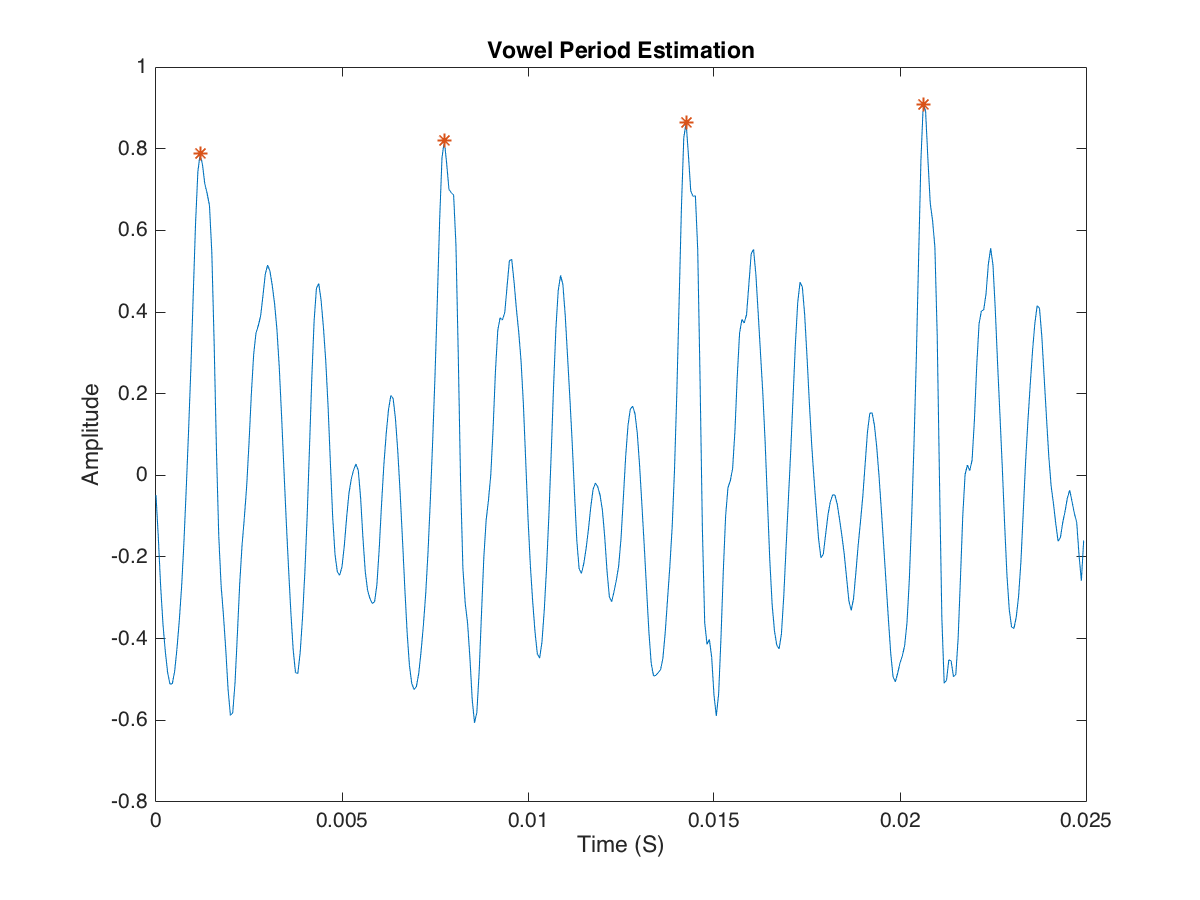
\includegraphics[width=.4\textheight]{vowel_period.png}
  \caption{The original vowel sample imported into Matlab.}
  \label{fig:vowel_period}
\end{figure}

\begin{figure}[h]
  \centering
    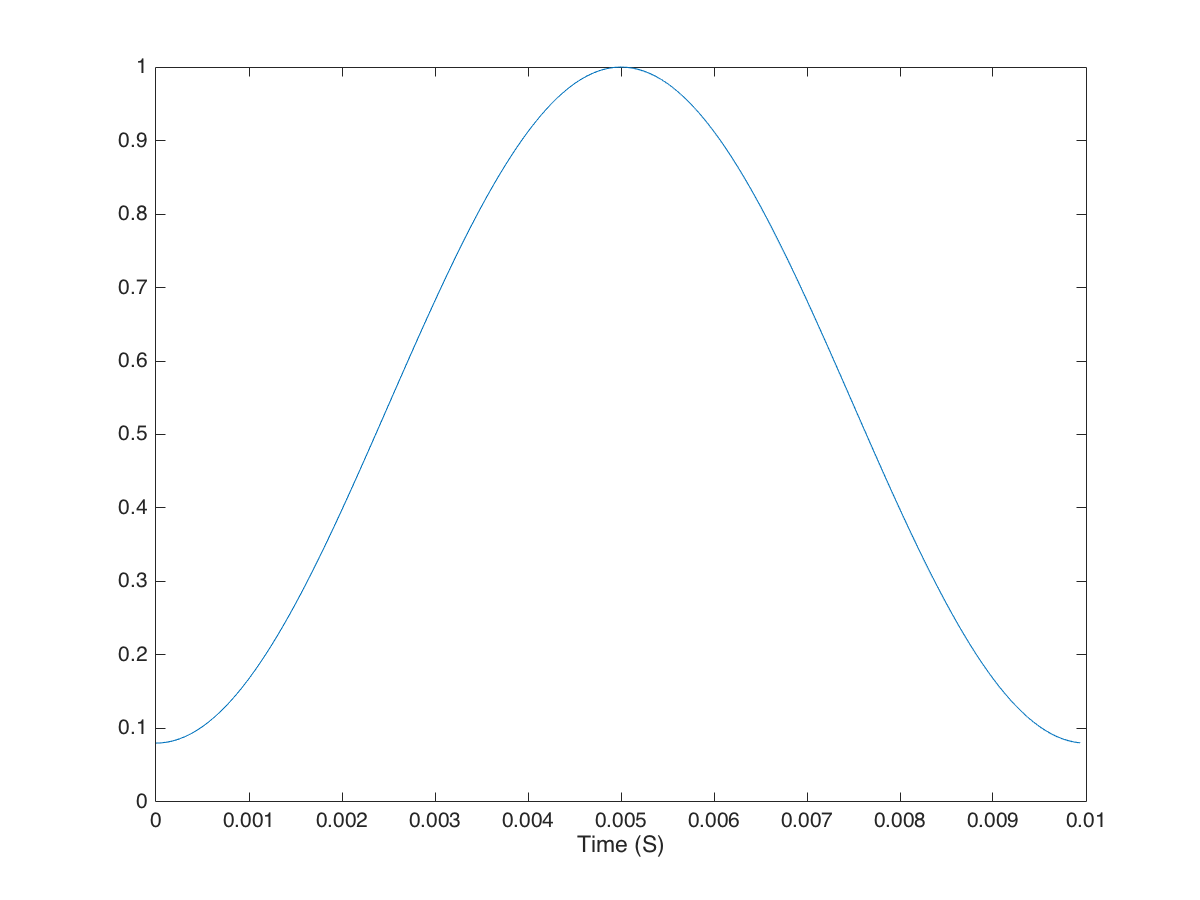
\includegraphics[width=.4\textheight]{hamming_window.png}
  \caption{Hamming window with width of 10 ms.}
  \label{fig:hamming_window}
\end{figure}
\begin{figure}[h]
  \centering
    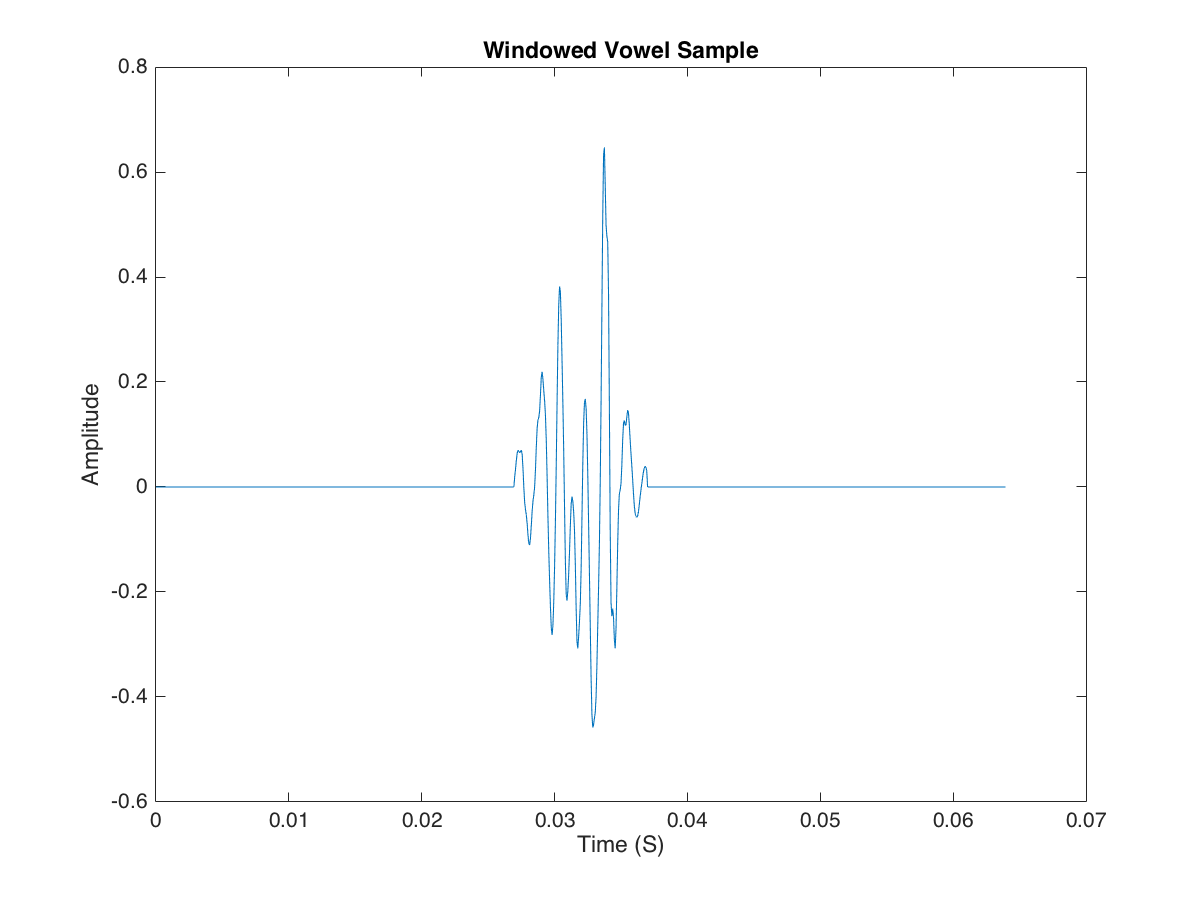
\includegraphics[width=.4\textheight]{vowel_windowed.png}
  \caption{Vowel sample after windowing with a hamming window of 25 ms.}
  \label{fig:vowel_windowed}
\end{figure}
Given this we can generate a dB spectrum of the windowed vowel sample using the Matlab FFT function. [Figs~\ref{fig:vowel_spec_win_10},~\ref{fig:vowel_spec_win_25}]
\begin{figure}[h]
  \centering
    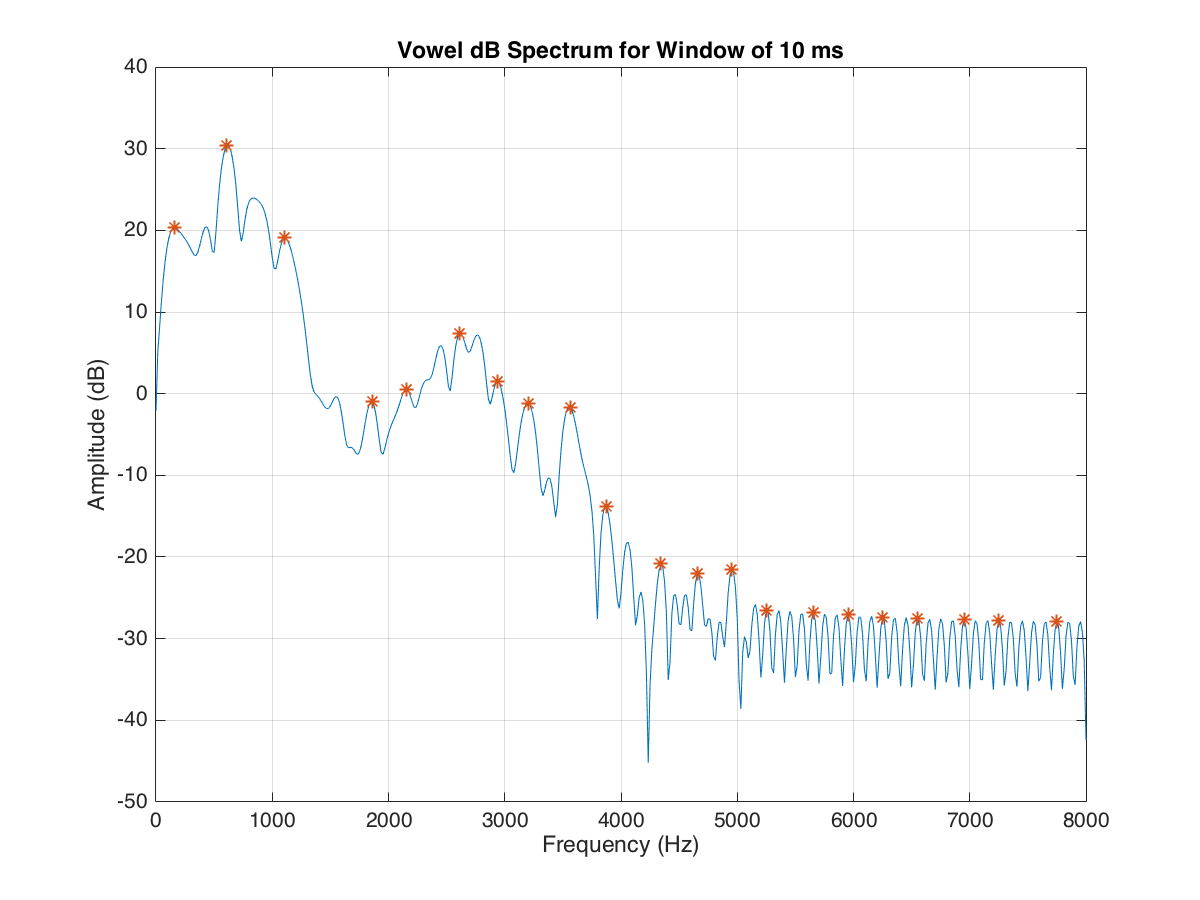
\includegraphics[width=.4\textheight]{vowel_spec_win_10.png}
  \caption{Spectrogram of vowel with a 10 ms hamming window.}
  \label{fig:vowel_spec_win_10}
\end{figure}
\begin{figure}[h]
  \centering
    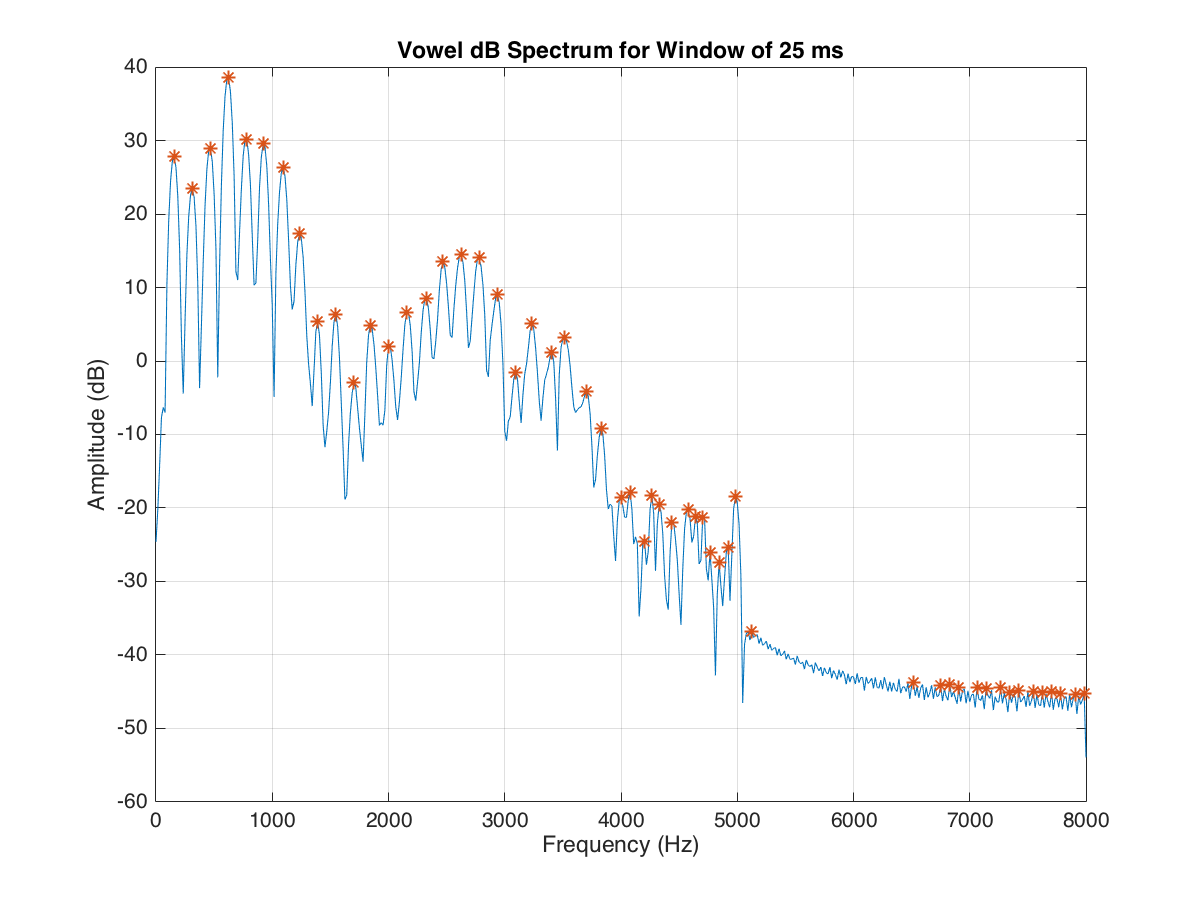
\includegraphics[width=.4\textheight]{vowel_spec_win_25.png}
  \caption{Spectrogram of vowel with a 25 ms hamming window. Notice the increased number of harmonics from the glottal impulses.}
  \label{fig:vowel_spec_win_25}
\end{figure}
\subsection{Pitch Estimation} % (fold)
\label{sub:pitch_estimation}
As can be seen in figures ~\ref{fig:vowel_period},~\ref{fig:vowel_spec_win_10},~and~\ref{fig:vowel_spec_win_25}, the relevant peaks for pitch estimation were found using the findpeaks function in matlab. The parameters for findpeaks varied between each instance since the have very different peak prominences and frequency. From the time domain signal, it is obvious from observation that there are 4 periods of the waveform present in the signal. Additionally, the 25ms window spectrum was much easier to estimate the fundamental period, since there are much more pronounced harmonics. Since we know what we're looking for, the findpeaks function was tweaked manually, and this will only work for the specific case here. In order to automate the process, we would need to look more closely at the spacing of the peaks found by findpeaks. For example by specifying a minimum peak spacing, we can filter out harmonics that are too high in frequency to be glottal harmonics. In the frequency spectrum the base pitch can be estimated as the first peak, or the average distance between peaks satisfying a certain spacing requirment. Table~\ref{tab:pitch_est} summarizes the results of the pitch estimation.
\begin{table}
\begin{tabular}{cc}
\hline
Source & Frequency\\
\hline
Waveform & 154.34\\
10ms Window Spectrum & 156.25Hz\\
25ms Window Spectrum & 156.25Hz\\
\hline
\end{tabular}
\label{tab:pitch_est}
\end{table}
% subsection pitch_estimation (end)
\FloatBarrier
\section{Vowel Synthesis} % (fold)
\label{sec:vowel_synthesis}
The vocal system can be approximated by the time convolution of a glottal wave train and an LTI filter. For our synthesis we assume that the filter whose frequency response can be described as an all pole filter described by Equation~\eqref{eq:all_pole_filt}. This is a reasonable approximation for the synthesis of vowels since they are typically long in duration with stable formants, and the vocal tract shape has certain resonances without significant anti-resonances. 
\begin{equation}\label{eq:all_pole_filt}
	H(z) = \prod\limits_{k=1}^{N}\frac{A}{(1-c_kz^{-1})(1-c_k^*z^{-1})}
\end{equation}
In order to simulate a glottal pulse, we use the rosenberg glottal model which is one of the simpler methods to generate the glottal excitation: \cite{shue2010interdependencies},~\cite{rosenberg_glottal}
\[
u_g(t) = 
\begin{cases}
	\frac{\alpha}{2}(1-cos(\frac{\pi t}{T_P})) &\text{, } 0 \leq t \leq T_P\\
	\alpha cos(\frac{\pi(t - T_P)}{2T_N}) &\text{, } T_P < t < T_P + T_N\\
	0 &\text{, Rest phase (glottal closure)}
\end{cases}
\]

Where $T_P$ is the time to maximal glottal amplitude (rise time), and $T_N$ is time from maximal glottal amplitude to closure (fall time). 

Instead of inventing the code from scratch, the a pre-existing matlab function was used to generate and sample this waveform. The rosenberg papers indicate that the duty cycle of the glottal pulse is slightly less than half, so we use a 45\% duty cycle for the glottal wave. [Fig~\ref{fig:glottal_wave_pulse}]. In order to generate the proper frequency of the pulse train, we build a vector of `delta' functions in matlab (ones) and convolve with the single glottal pulse to generate our excitation waveform. A subset of the entire wave train is shown in Figure~\ref{fig:glottal_wave_train}. 
\begin{figure}[h]
  \centering
    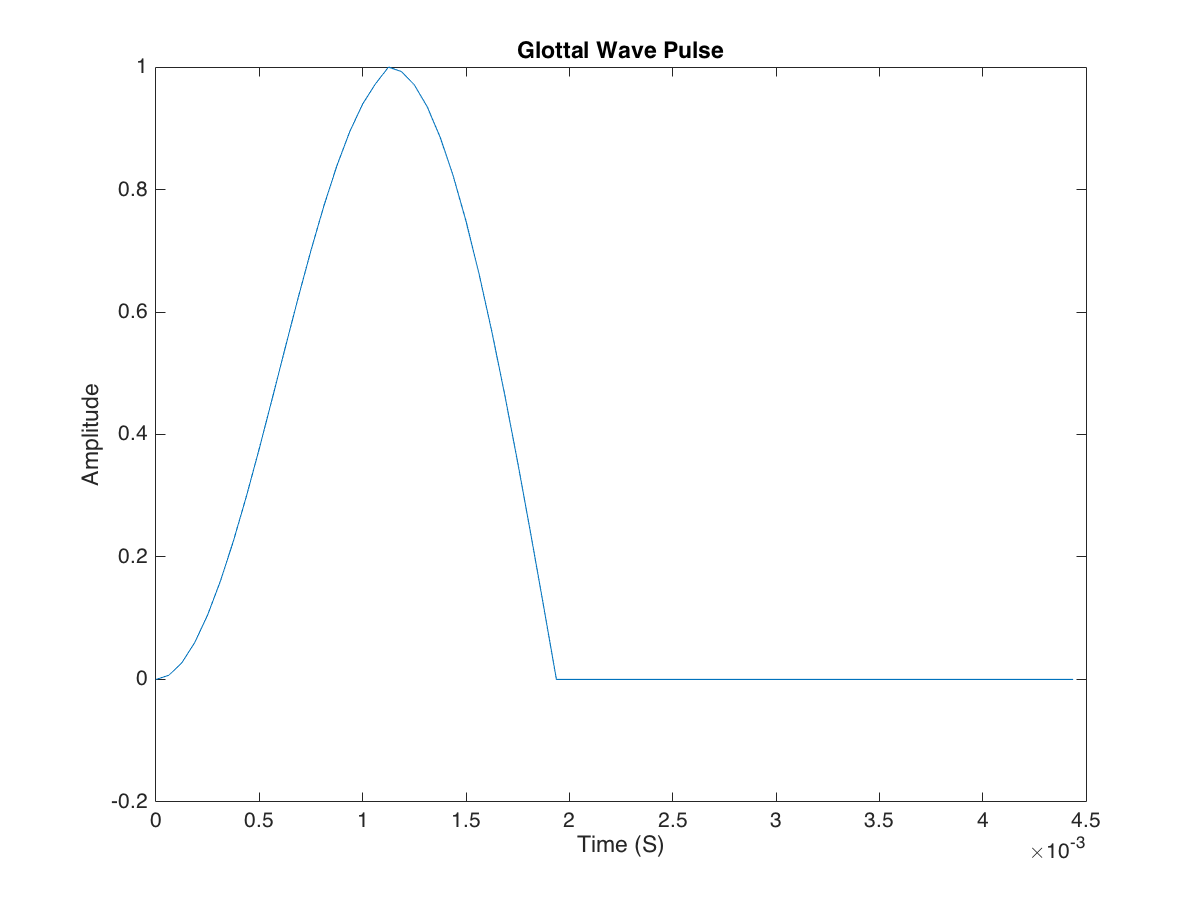
\includegraphics[width=.4\textheight]{glottal_wave_pulse.png}
  \caption{A single glottal pulse as generated by the Rosenberg model.}
  \label{fig:glottal_wave_pulse}
\end{figure}
\begin{figure}[h]
  \centering
    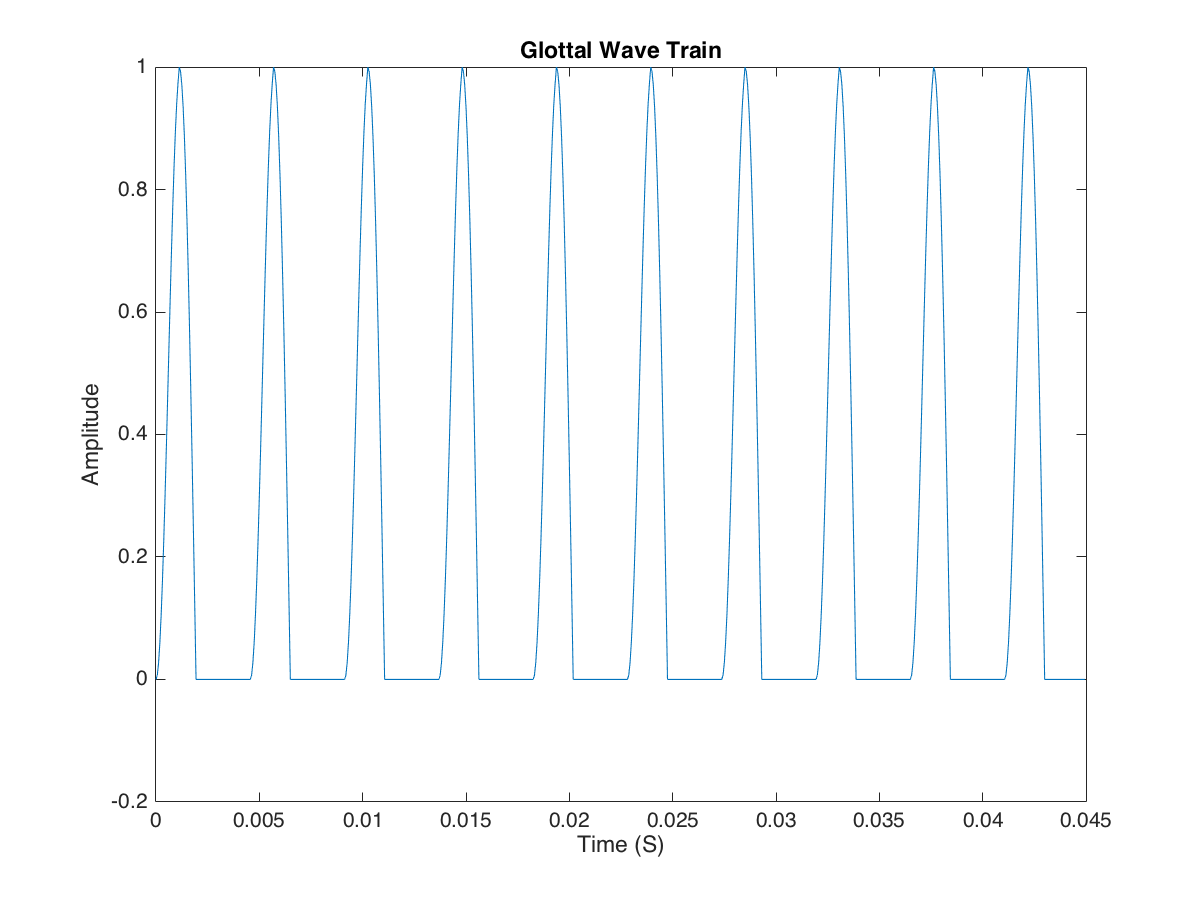
\includegraphics[width=.4\textheight]{glottal_wave_train.png}
  \caption{Glottal pulse train with ten pulses.}
  \label{fig:glottal_wave_train}
\end{figure}
Using the table from the Peterson and Barney '52 paper [\cite{peterson_barney_vowels}], the center frequencies for the female formants were used in the vocal model. In order to generate variability in the output vowels, we use a randomized collection of points within each vowel region. To do this, each vowel region was approximated with an ellipse with a center as defined by the table, and a rotation and sizing appropriate for the region being covered. To aid in the region selection process, the ellipses were plotted over Figure~\ref{fig:vowel_formants}
\begin{figure}[h]
  \centering
    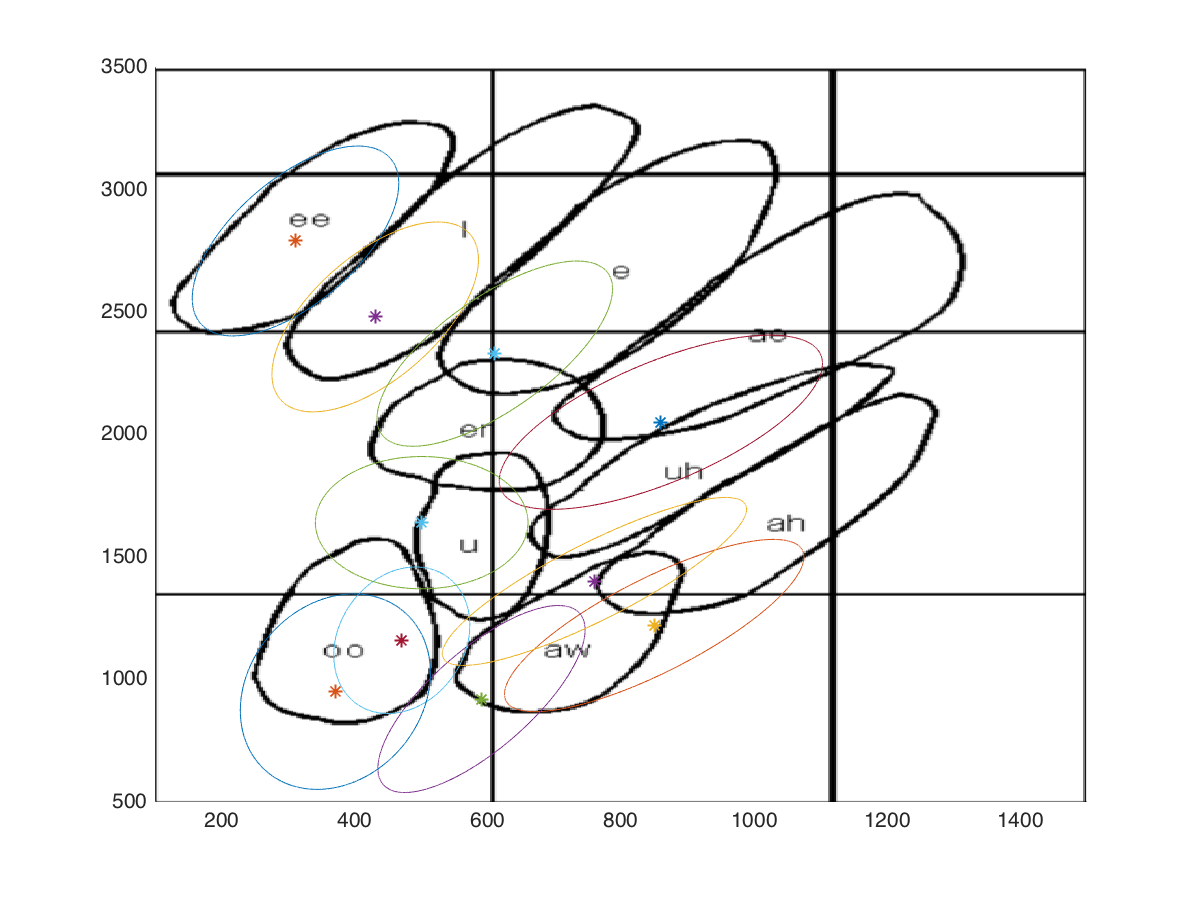
\includegraphics[width=.4\textheight]{vowel_formants.png}
  \caption{Vowel regions with female vowel frequency centers. As can be seen, the average vowel regions and female vowel regions do not necessarily overlap.}
  \label{fig:vowel_formants}
\end{figure}
As can be seen from Figure~\ref{fig:vowel_formants} the vowel regions do not necessarily match up well with the average vowel regions. However the vowels were distinctive enough that this was considered a non-issue. A 2D uniform distribution with dimensions of the major and minor ellipse axes was mapped to the proper ellipse shape, and then rotated and translated into the proper coordinate range using a rotation matrix. [Figure~\ref{fig:vowel_formant_regions}] The number of random points generated per vowel can be specified by the user, as well as the specific vowel for which formants are to be generated. 
\begin{figure}[h]
  \centering
    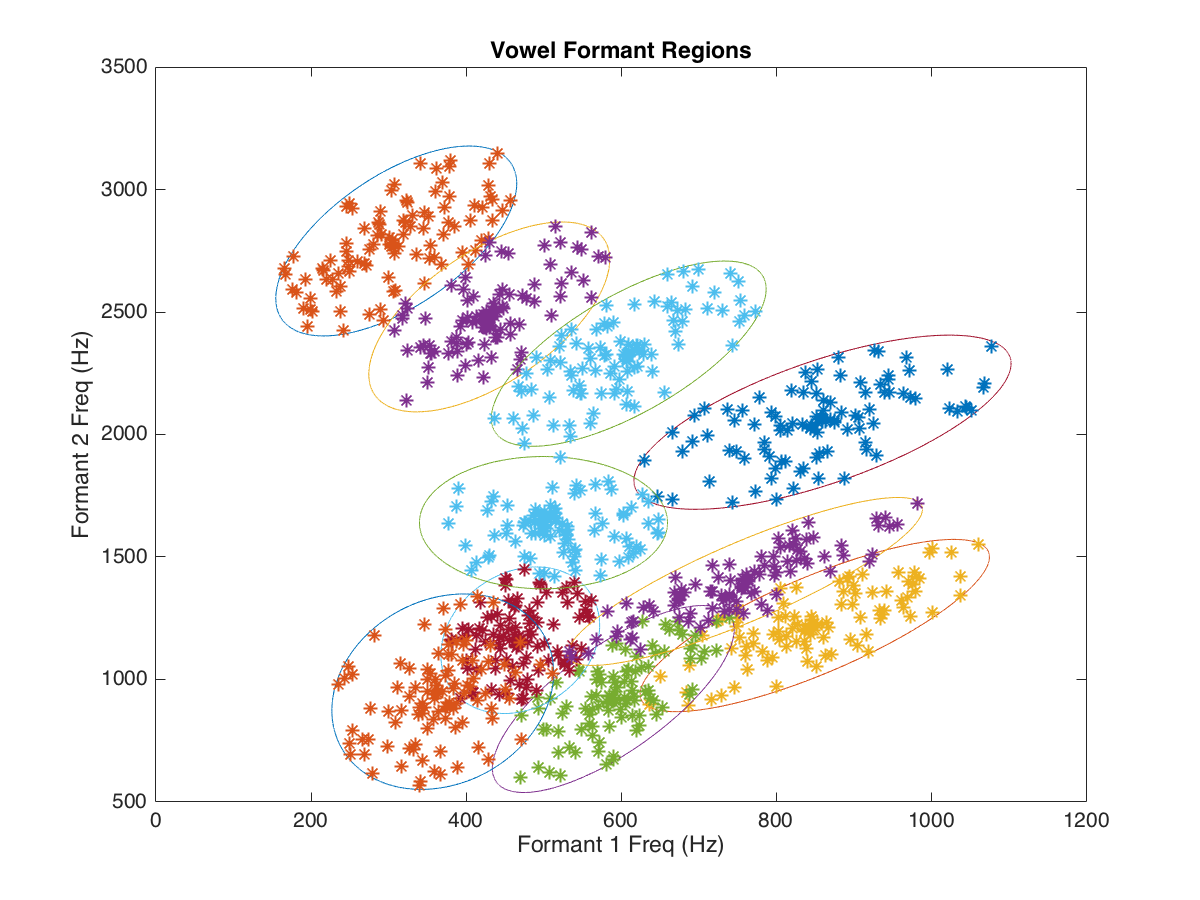
\includegraphics[width=.4\textheight]{vowel_formant_regions.png}
  \caption{This figure shows each of the vowel regions with 100 randomly generated points within each region.}
  \label{fig:vowel_formant_regions}
\end{figure}
Having satisfied the requirement for variability in the formant frequencies we generate the filter roots by computing the scaled frequency and its complex conjugate in the Z domain. This is necessary to fully describe the roots of the filter as defined in Equation~\eqref{eq:all_pole_filt}. When generating the roots of the filter we also scale the values by 0.9 to avoid placing poles on the unit circle. Placing the poles on the unit circle would cause the filter to be unstable since there will be infinite gain ath that frequency. The roots are then expanded into filter coefficients using the poly function.
Using the freqz function we can evaluate a sample set of filters generated by the matlab code. [Figure~\ref{fig:vowel_filter_response}]

\begin{figure}[h]
  \centering
    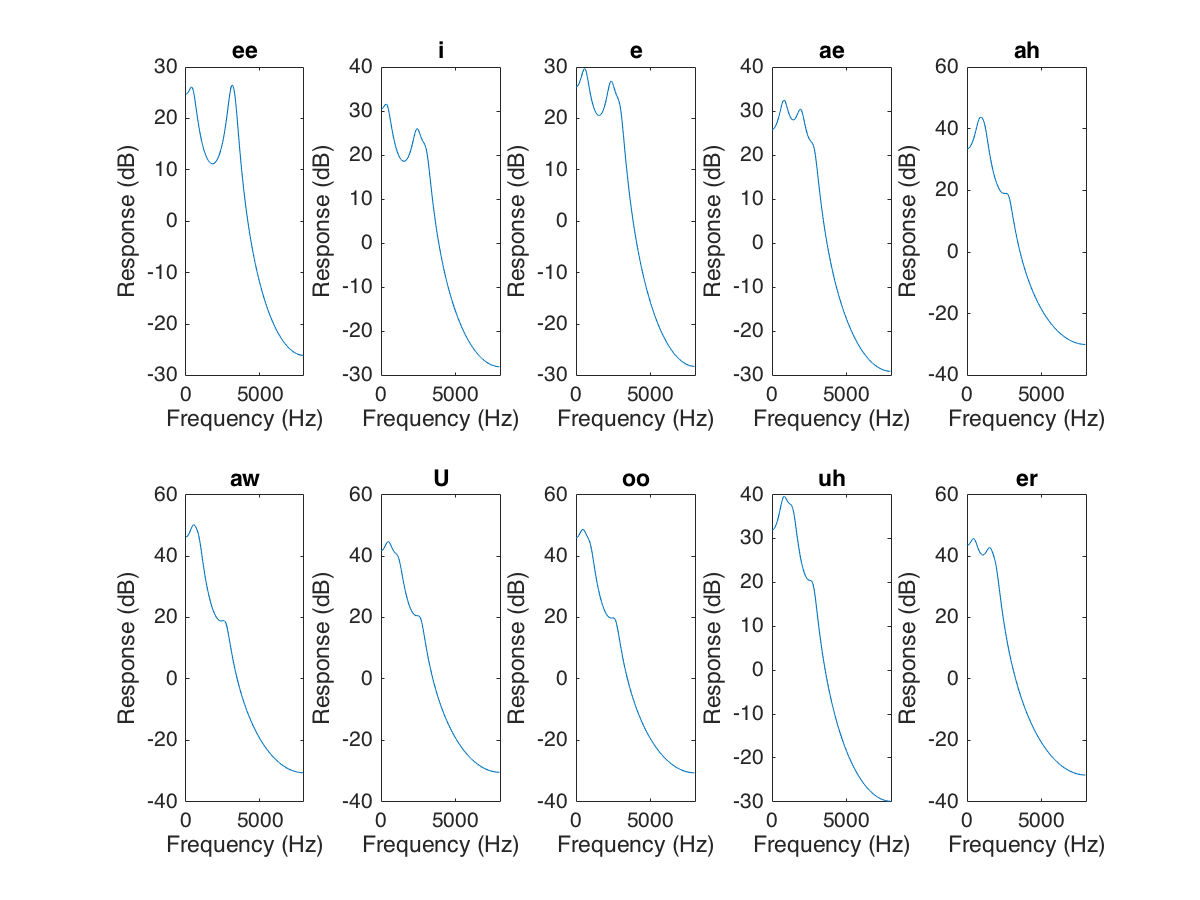
\includegraphics[width=.4\textheight]{vowel_filter_response.png}
  \caption{Frequency responses in dB a sample of each vowel.}
  \label{fig:vowel_filter_response}
\end{figure}

Thus having generated the two necessary elements of the system, the glottal pulse train and the filter, finally we can generate a vowel using a filtering function in matlab. The fuction filtfilt was chosen to eliminate any phase distortions that may arrise from the filter implementation. Filtfilt is phase invariant since it filters the input signal twice, once in its original orientation, and then the time reversed output of the original filtering operation. This allows us to remove the phase distortions caused by the filter which is desirable since excessive or discontinuous phase variations in speech signals can destroy the information in the waveform. 
\begin{figure}[h]
  \centering
    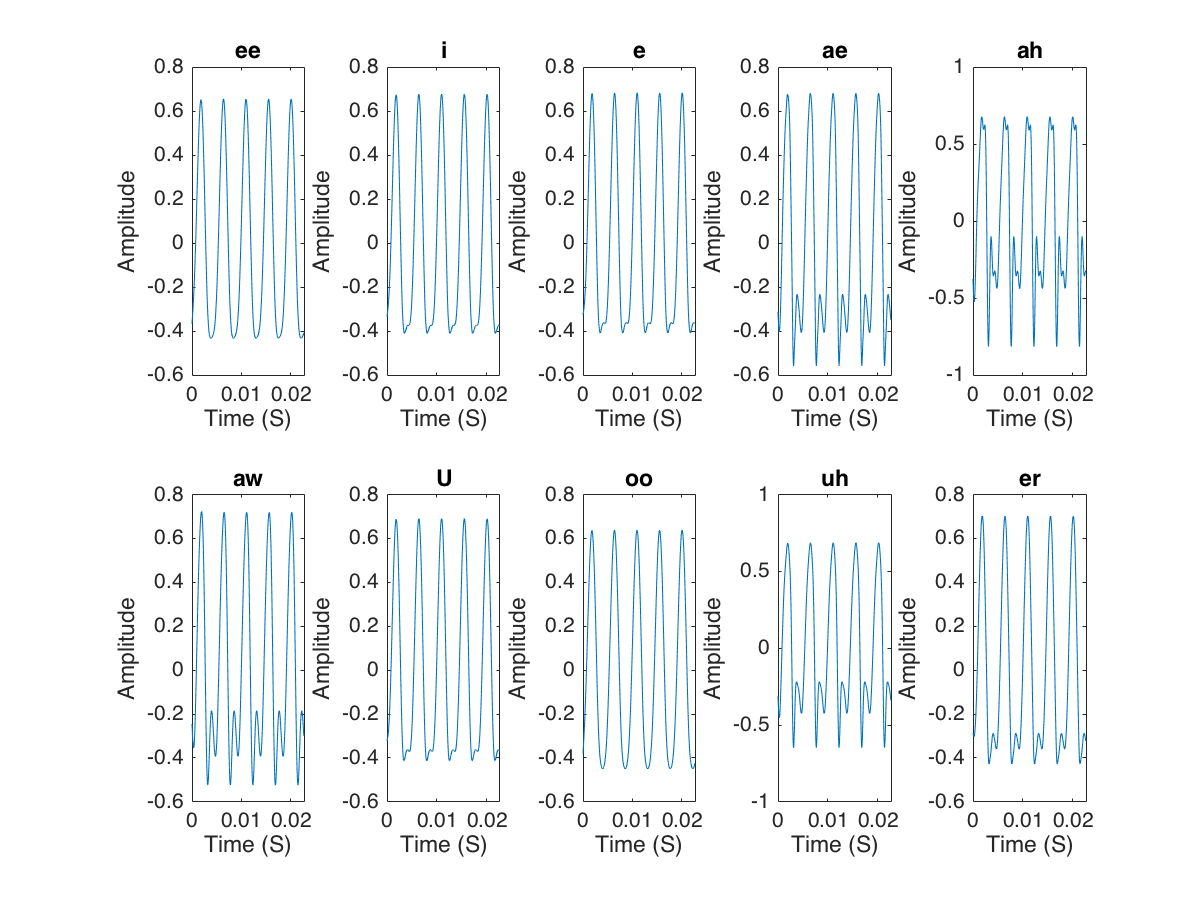
\includegraphics[width=.6\textwidth]{vowels_time.png}
  \caption{Time domain representation of our generated vowels.}
  \label{fig:vowels_time}
\end{figure}

\begin{figure}[h]
  \centering
    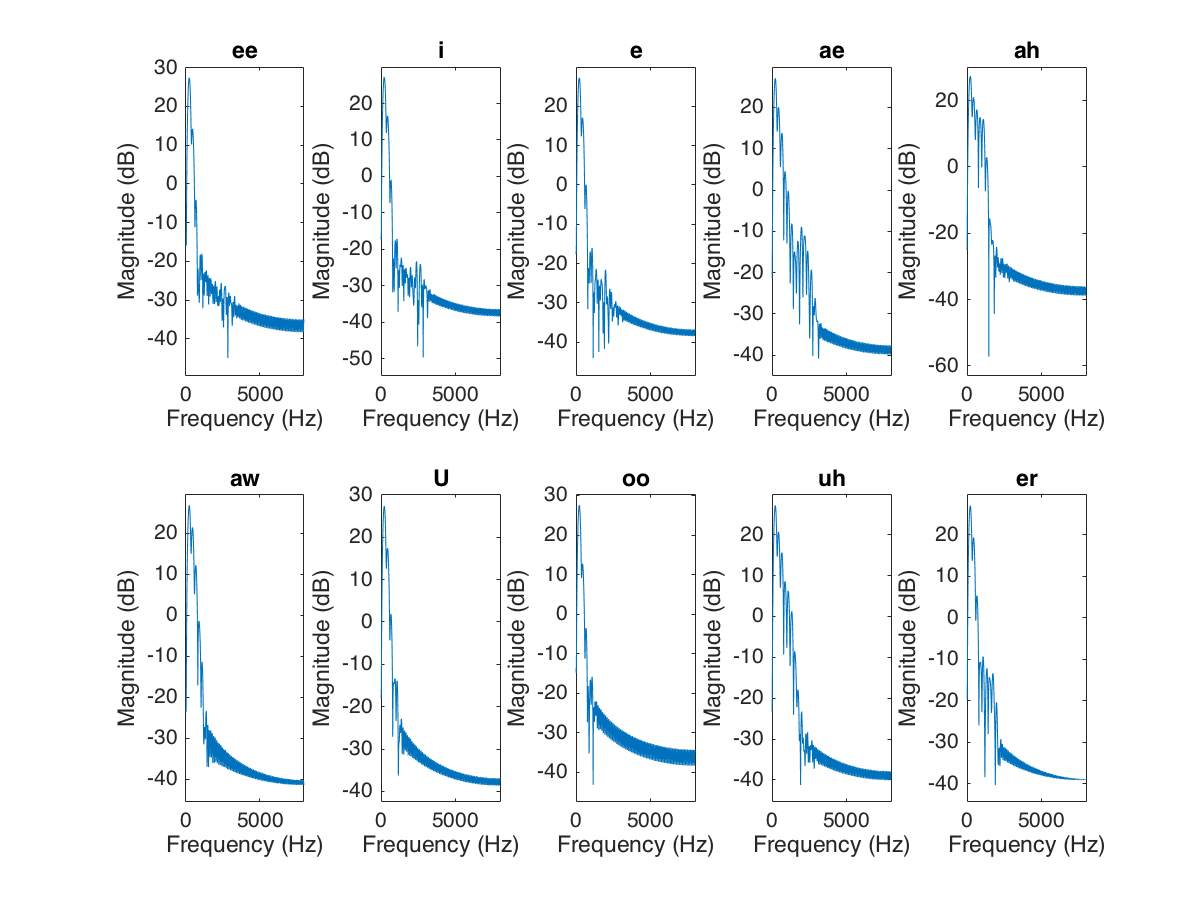
\includegraphics[width=.6\textwidth]{vowels_freq.png}
  \caption{Frequency domain representation of generated vowels.}
  \label{fig:vowels_freq}
\end{figure}
\begin{figure}[h]
  \centering
    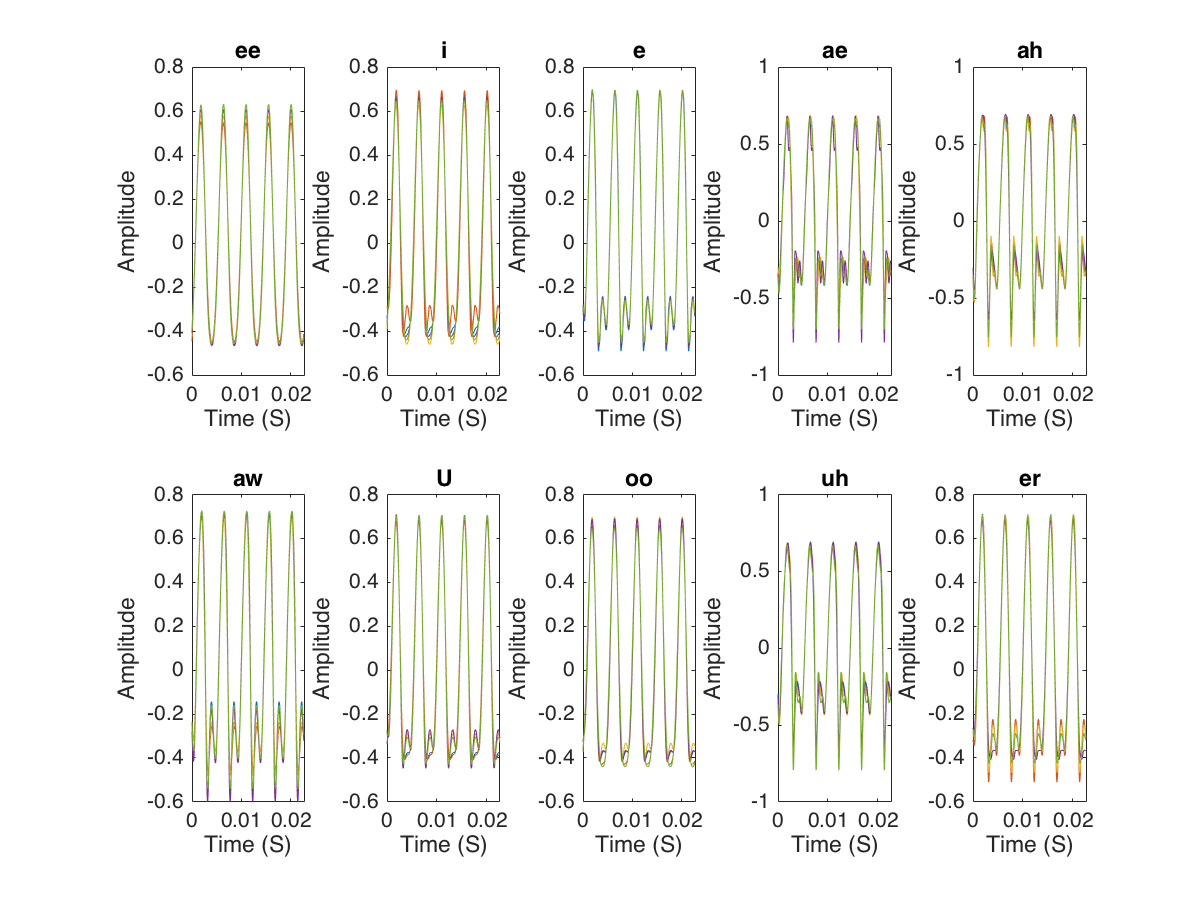
\includegraphics[width=.6\textwidth]{vowel_variation_time.png}
  \caption{Time domain representation of five variations of the same vowel.}
  \label{fig:vowel_variation_time}
\end{figure}
\begin{figure}[h]
  \centering
    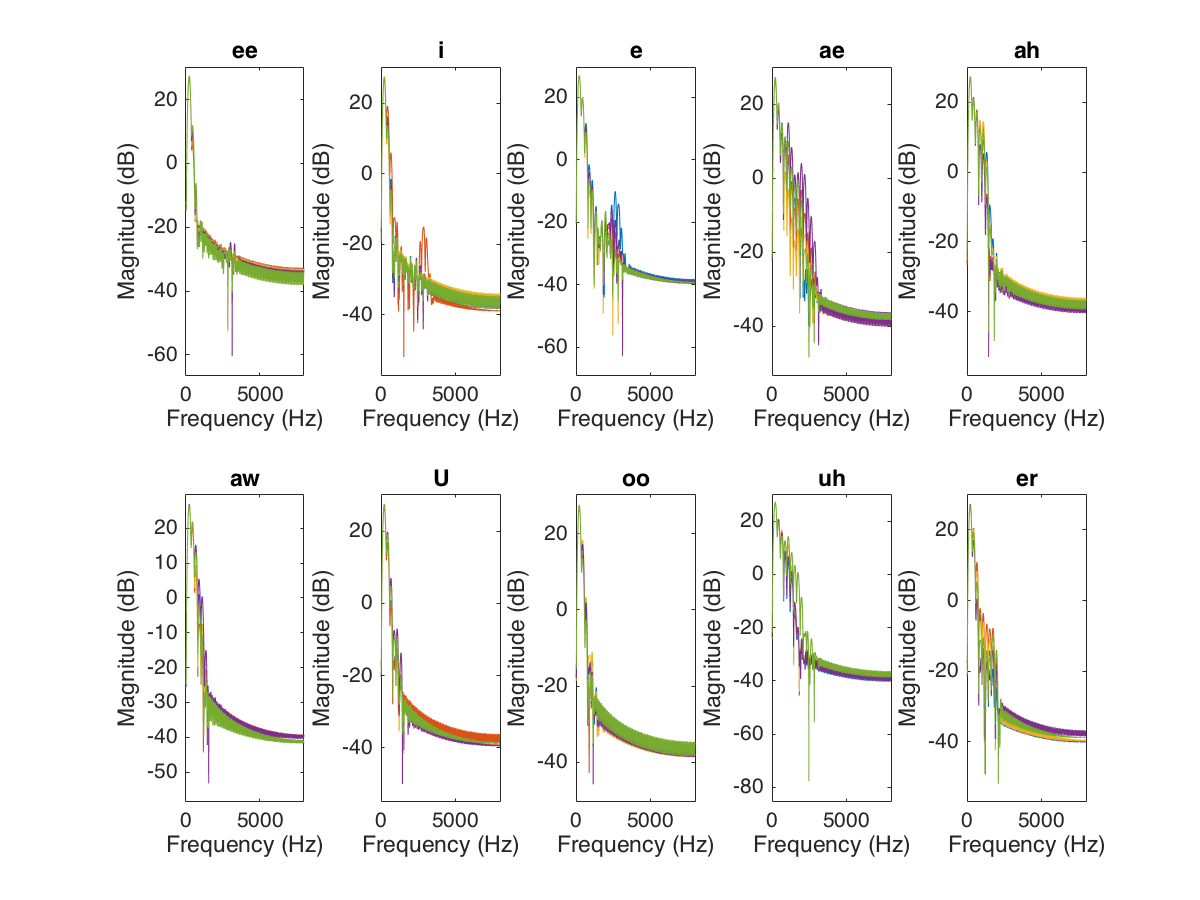
\includegraphics[width=.6\textwidth]{vowel_variation_freq.png}
  \caption{Frequency domain representation of five variations of the same vowel.}
  \label{fig:vowel_variation_freq}
\end{figure}
Using the matlab code written, each vowel sound was successfully synthesized using randomized formant combinations. As can be seen in figures~\ref{fig:vowel_variation_time},~and~\ref{fig:vowel_variation_freq} the random variations in the formant frequencies was able to generate noticable variation in the output. Listening to the vowel sounds it was also confirmed aurally that each vowel had differences that were identifiable. After listening to the sound of the formants and experimenting with adding a third formant, the third center formant frequency for each vowel was added to the filter generation step. No variability was introduced to this value since the Peterson and Barney paper did not include such information. This significantly increased sound quality and made the vowels more easily distinguishable and more natural sounding. Obviously the more information used to generate the signal the more realistic the synthesized waveform will sound. Another easy improvement would be to slightly vary the glottal waveform parameters, and add noise to the wave train to make the signal more realistic. In addition, the delta functions used to generate the final wave train should also have time variability to simulate shimmer and natural fluctuations in pitch. However, adding this information will increase the complexity of the signal construction and how much space is required to save the generated waveforms since higher formant frequencies require higher sampling rates. 
% section vowel_synthesis (end)
\pagebreak
\bibliographystyle{plain}
\bibliography{main}
\end{document}
